\documentclass[12pt,letterpaper]{article}
\newcommand{\sethead}[5]{
	\lhead{\textit{#1}}
	\rhead{#2\\#3\\#4\\#5}
}
\usepackage[utf8]{inputenc}
\usepackage{fancyhdr}
\usepackage{setspace}
\usepackage{geometry}
\newgeometry{top=1in,bottom=1.5in,left=1in,right=1in}
\usepackage{graphicx}
\usepackage{amsmath}
\usepackage{amsfonts}
\usepackage{listings}
\usepackage{xcolor}

\lstset{
	frame=tb,
    tabsize=4,
    showstringspaces=false,
    numbers=left,
    commentstyle=\color{green},
    keywordstyle=\color{blue},
    stringstyle=\color{red}
}

\pagestyle{fancy}

\begin{document}
    \newlength{\saveparindent}
	\setlength{\saveparindent}{\parindent}
	\raggedright
	\setlength{\parindent}{\saveparindent}
	\sethead{Homework 2}{Adrian Lu, Josh Kuroda, \& Edward Seim}{CMSI 284}{Toal}{March 5, 2015}
    
	\doublespacing
    \begin{center}
    \end{center}
    \begin{enumerate}
        \item %1
        	AND, OR, NOT: X = A + BC, Y = AC + \={A}\={B}
            \newline
            NAND: X = (\={A}$\overline{BC}$)', Y = ((\={A}\={B})'$\overline{AC}$)'
        \item %2
            The circuit is as follows:\newline 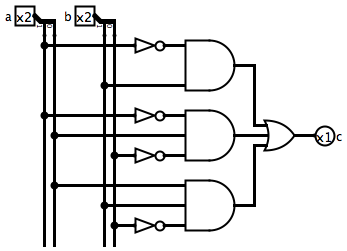
\includegraphics{Circuit1.png}
        \item %3
        	\begin{enumerate}
            	\item 
                	AND with AAAAAAAA
                \item 
                	OR with 00000007
                \item 
                	AND with 00000007
                \item 
                	AND with 00000000
                    \newline
                    OR with FFFFFFFF
                \item 
                	XOR with C0000000
                \item 
                	AND with FFFFFFF8
            \end{enumerate}
        
        \pagebreak
        \item %4
        	\begin{lstlisting}[language=C, caption={0 - 255}]
            JUMP	start
    add:	1
    cur:	0
    up:		256
    start:  LOAD	cur
    		OUT		0x8
            ADD		add
            STORE	cur
            SUB 	up
            JLZ 	start
    end:	JUMP	end
            \end{lstlisting}
            
        \item %5
        	\begin{lstlisting}[language=C, caption={0 - 255}]
		    0000	C0000004
    		0001	00000001 
    		0002	00000000 
    		0003	00000100 
    	    0004	00000002 
    		0005	30000008 
            0006	40000001 
            0007	10000002 
            0008 	50000003 
            0009	E0000004 
    		000A	C000000A 
            \end{lstlisting}
            
        \item %6
        	\begin{lstlisting}[language=C, caption={GCD}]
            JUMP	start
    num1:	0
    num2:	0
    hold:	0
    start:  IN		0x100
    		STORE	num1
            IN		0x100
            STORE	num2
	loop:	LOAD	num1
    		STORE	hold
    		LOAD	num2
    		MOD		num1
            STORE	num1
            LOAD	hold
            STORE	num2
            LOAD	num1
            JGZ		loop
    out:	LOAD	num2
    		OUT		0x200
    end:	JUMP	end
            \end{lstlisting}
        
        \pagebreak
        \item %7
        	\begin{lstlisting}[language=C, caption={Swap Accumulator and 0x222A}]
            JUMP	start
    acc:	0
    mem:	0
    start:  STORE	acc
    		LOAD	0x222A
            STORE	mem
            LOAD	acc
            STORE	0x222A
            LOAD	mem
            \end{lstlisting}
            
        \item %8
        	\begin{lstlisting}[language=C, caption={Jump}]
            JZ		0x837BBE1
            JGZ		0x837BBE1
            \end{lstlisting}
        
    \end{enumerate}
    
\end{document}